\chapter{Multihoming and Redundancy}

\label{Multihoming and Redundancy}
In Section one we have created two different networks and connected them through collision domain I. It worked fine however integrating that in real life most probably will cause a lot of problems as we will have a single point of failure. In this section we will work on this problem by introducing third Area called AS 3 to have another route in case failure occurs at collision domain I.

Our goal will be \ref{fig:2.1}
\begin{figure}[H]
\centering
  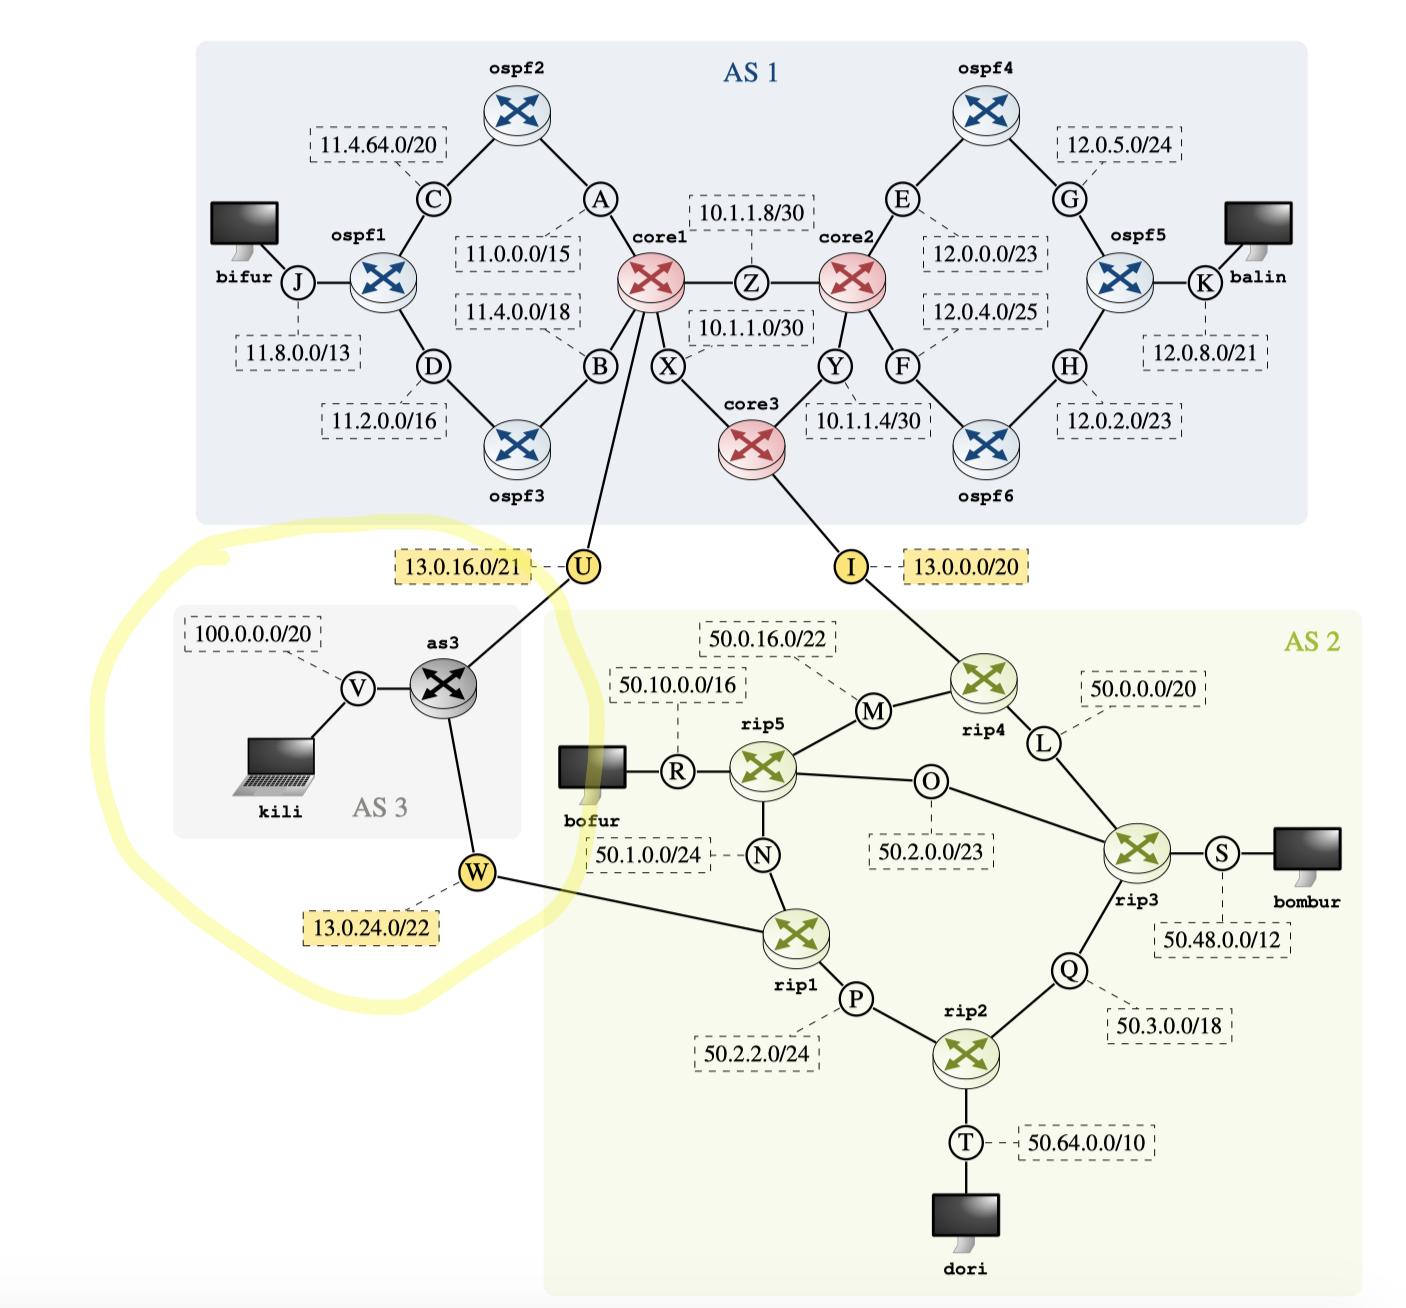
\includegraphics[width=0.73\textwidth]{Images/NetERoute.png}
  \caption{Our Network with extra route}
  \label{fig:2.1}
\end{figure}

\section{Structuring AS3 network to offer another route}

Lets Now Go through steps to create the extra area in  figure \ref{fig:2.1}
\subsection{Configure BGB router \textbf{as3} and Connect as3 with core1 through collision domain U and Connect as3 with rip1 through collision domain W}

\begin{figure}[H]
  \centering
  \begin{minipage}[b]{0.45\textwidth}
    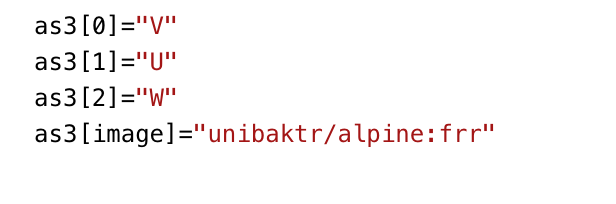
\includegraphics[width=\textwidth]{Images/as3 LapConf.png}
    \caption{Adding As3 in labConf file. and connect it with three collison domains V, U and W}
  \end{minipage}
  \hfill
  \begin{minipage}[b]{0.45\textwidth}
    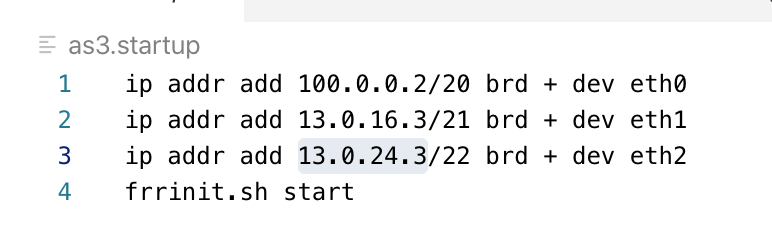
\includegraphics[width=\textwidth]{Images/as3Setup.png}
    \caption{As3 startup file and configure address for each collision domain.}
  \end{minipage}
\end{figure}
\begin{figure}[H]
\centering
 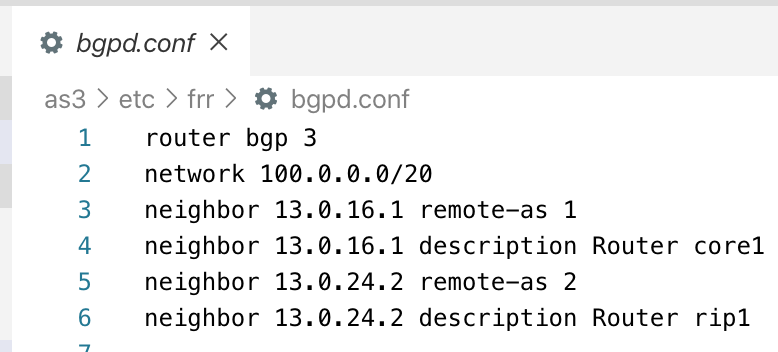
\includegraphics[width=\textwidth]{Images/as3BGPD.png}
 \caption{Setuping as3 router as BGP router.}
  \label{fig:2.4}
\end{figure}


\section{Add kili to the new network and connect it to bgp router as3}

\begin{figure}[H]
  \centering
  \begin{minipage}[b]{0.45\textwidth}
    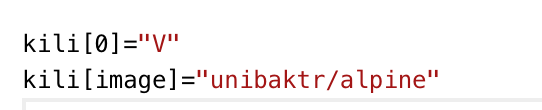
\includegraphics[width=\textwidth]{Images/kiliConf.png}
    \caption{Adding kili to labConf file and attaching it to collision domain V.}
  \end{minipage}
  \hfill
  \begin{minipage}[b]{0.45\textwidth}
    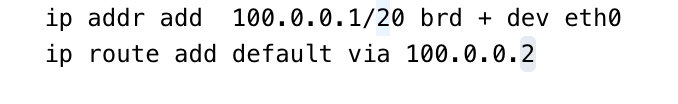
\includegraphics[width=\textwidth]{Images/kiliStartUp.png}
    \caption{Configuring kili startup file and setting its default router to be as3.}
  \end{minipage}
\end{figure}

\section{Connecting network 1 with the new network by connecting core 1 to as3 bgp router through U interface and configuring IBGP in area one for core 1 and core 3}

\begin{figure}[H]
  \centering
  \begin{minipage}[b]{0.45\textwidth}
    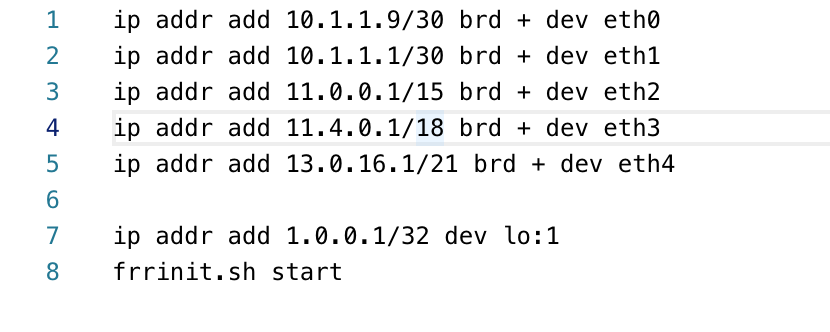
\includegraphics[width=\textwidth]{Images/core1Update.png}
    \caption{Updating Core1 startup file.}
  \end{minipage}
  \hfill
  \begin{minipage}[b]{0.45\textwidth}
    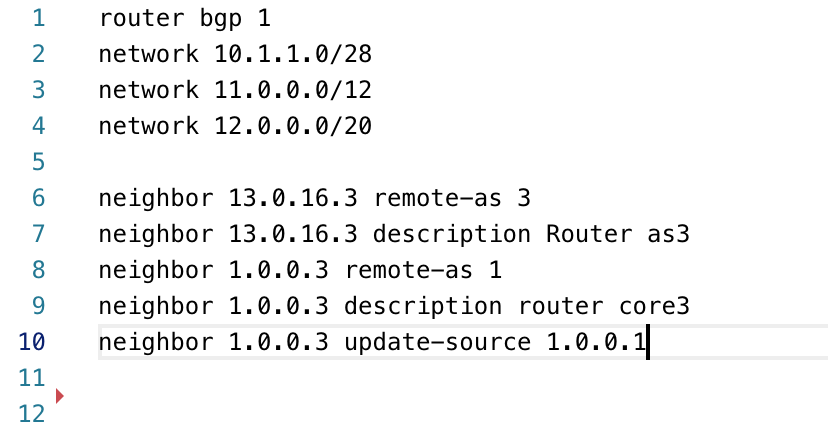
\includegraphics[width=\textwidth]{Images/as3Core1.png}
    \caption{Configuring BGP to core1 and configuring IBGP.}
  \end{minipage}
\end{figure}

\begin{figure}[H]
\centering
  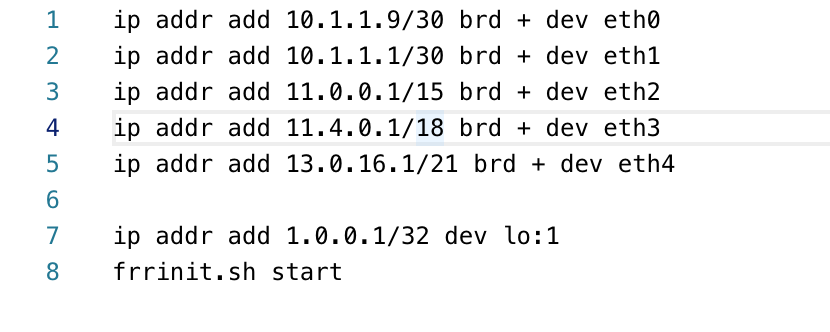
\includegraphics[width=0.73\textwidth]{Images/core1Update.png}
  \caption{Adding iBGP in core3 bgp configurations}
  \label{fig:2.10}
\end{figure}

\section{Connecting network 2 with the new network by connecting rip3 to as3 bgp router through W interface.}

\begin{figure}[H]
  \centering
  \begin{minipage}[b]{0.45\textwidth}
    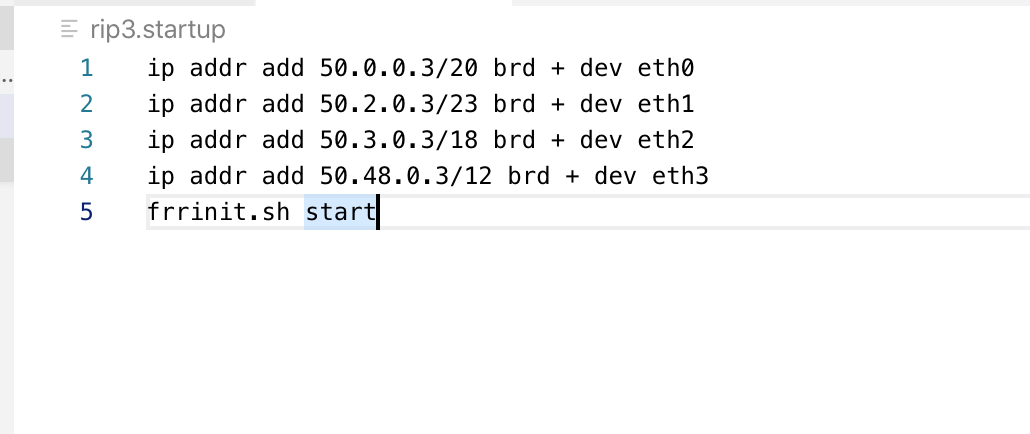
\includegraphics[width=\textwidth]{Images/rip3Update.png}
    \caption{Updating Rip3 startup file.}
  \end{minipage}
  \hfill
  \begin{minipage}[b]{0.45\textwidth}
    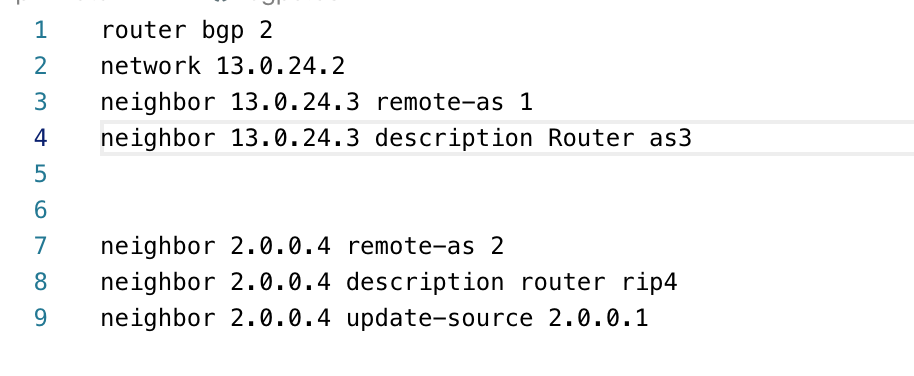
\includegraphics[width=\textwidth]{Images/rip3As3.png}
    \caption{Updating Rip3 bgp configurations and configuring IBGP}
  \end{minipage}
\end{figure}

\begin{figure}[H]
\centering
  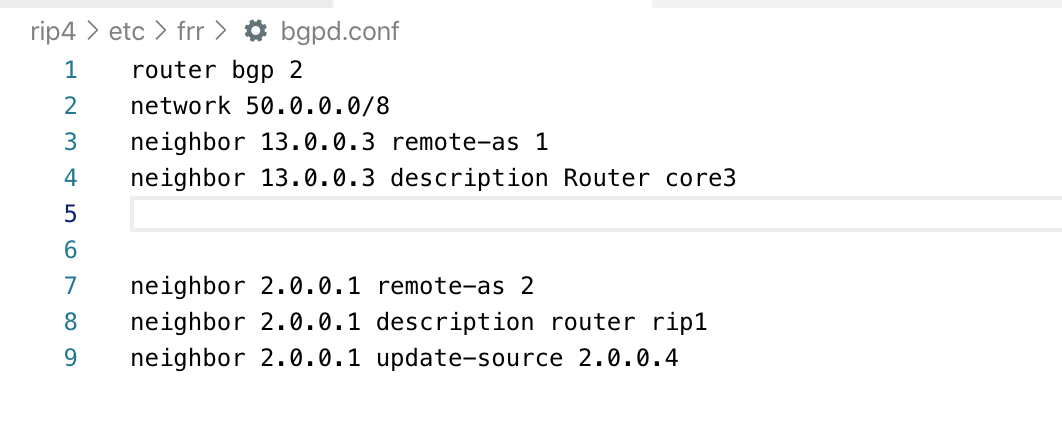
\includegraphics[width=0.73\textwidth]{Images/rip4Upd.png}
  \caption{Adding iBGP in rip4 bgp configurations}
  \label{fig:2.14}
\end{figure}



\section{Testing connection between neworks}
\subsection{Sending from Area 1 to Area 2 and Area 3}

\begin{figure}[H]
  \centering
  \begin{minipage}[b]{0.45\textwidth}
    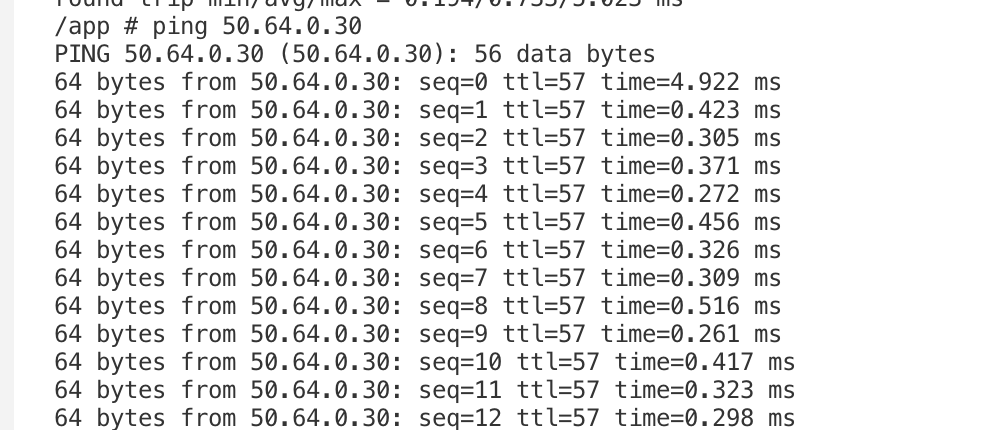
\includegraphics[width=\textwidth]{Images/bifur2Dori.png}
    \caption{pinging from bifur to dori.}
  \end{minipage}
  \hfill
  \begin{minipage}[b]{0.45\textwidth}
    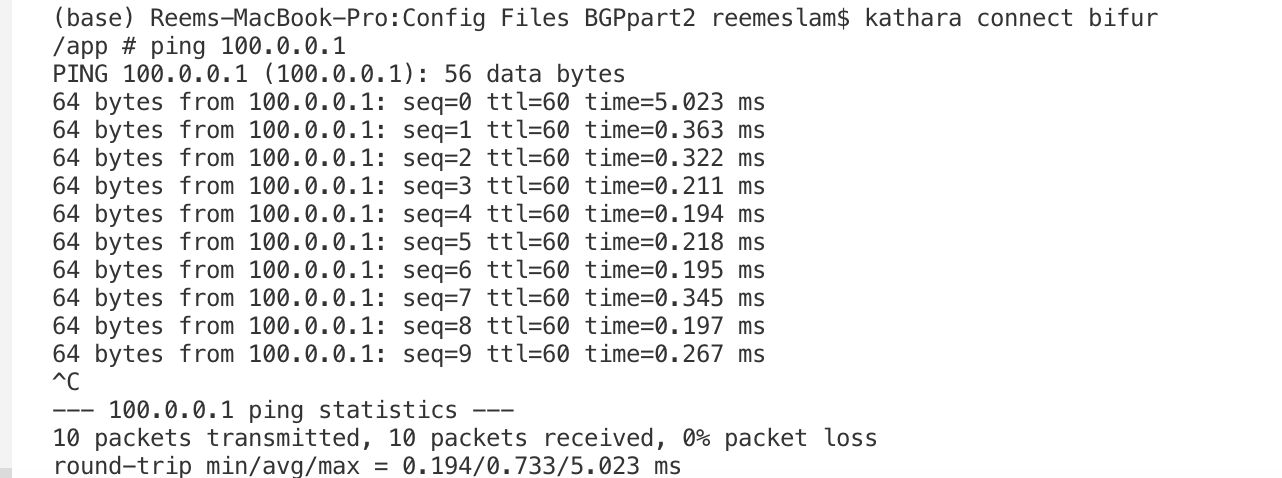
\includegraphics[width=\textwidth]{Images/bifur2kili.png}
    \caption{pinging from bifur to kili.}
  \end{minipage}
\end{figure}

\subsection{Sending from Area 2 to Area 1 and Area 3}

\begin{figure}[H]
  \centering
  \begin{minipage}[b]{0.45\textwidth}
    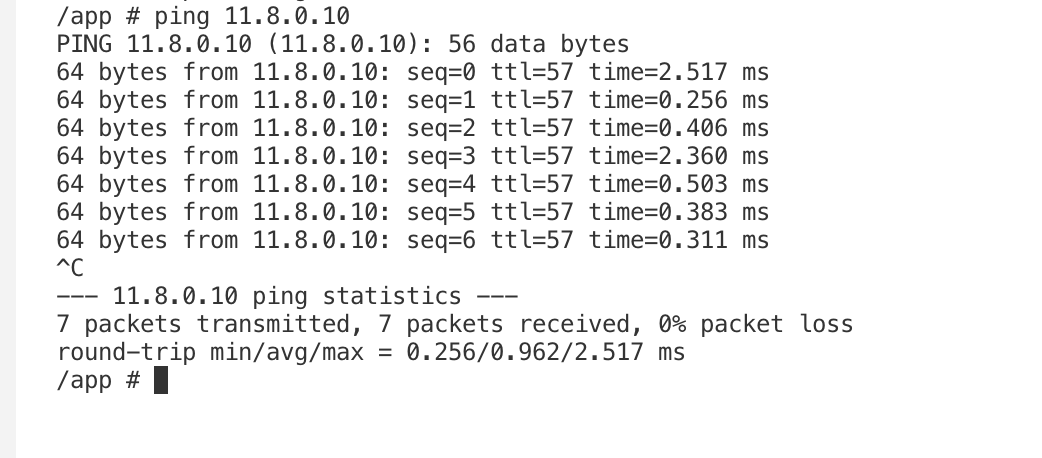
\includegraphics[width=\textwidth]{Images/dori2bifur.png}
    \caption{pinging from dori to bifur.}
  \end{minipage}
  \hfill
  \begin{minipage}[b]{0.45\textwidth}
    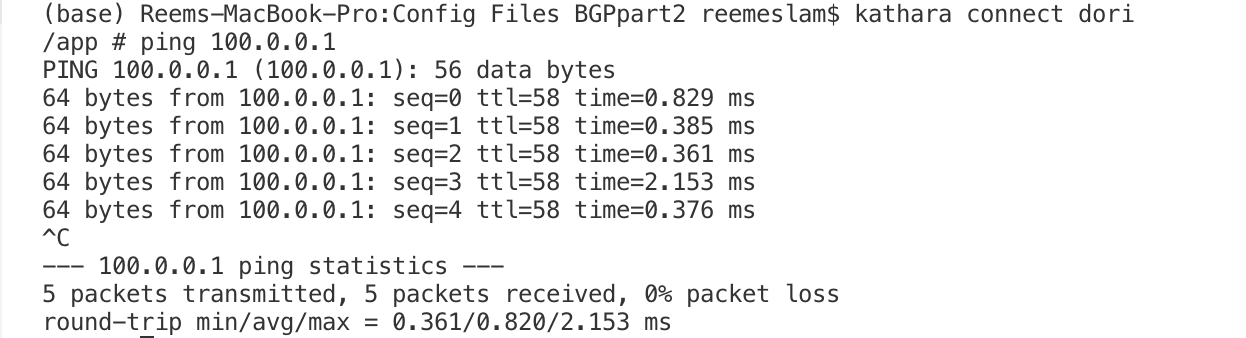
\includegraphics[width=\textwidth]{Images/dori2kili.png}
    \caption{pinging from dori to kili.}
  \end{minipage}
\end{figure}

\subsection{Sending from Area 3 to Area 2 and Area 1}

\begin{figure}[H]
  \centering
  \begin{minipage}[b]{0.45\textwidth}
    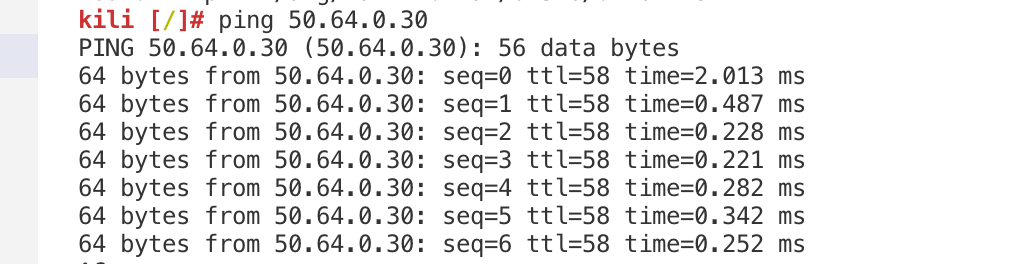
\includegraphics[width=\textwidth]{Images/kili2dori.png}
    \caption{pinging from kili to dori.}
  \end{minipage}
  \hfill
  \begin{minipage}[b]{0.45\textwidth}
    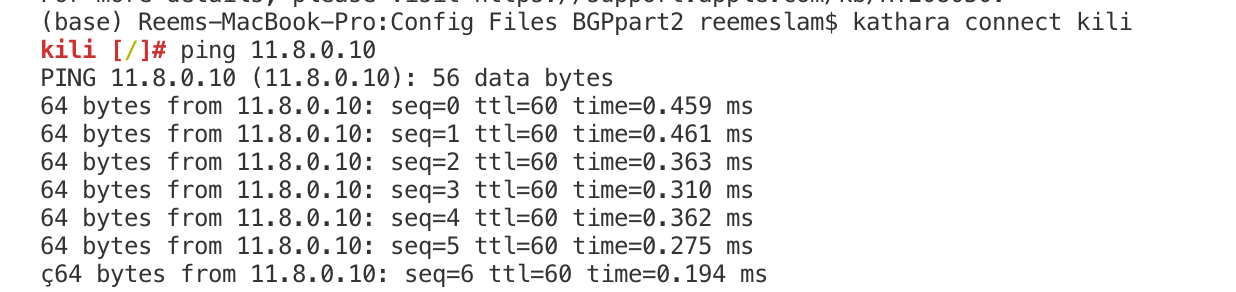
\includegraphics[width=\textwidth]{Images/kili2bifur.png}
    \caption{pinging from kili to bifur.}
  \end{minipage}
\end{figure}

\section{Evaluation of whole network on the path from bombur to balin.}

\subsection{Determine the path between both nodes with traceroute.}

\begin{figure}[H]
\centering
  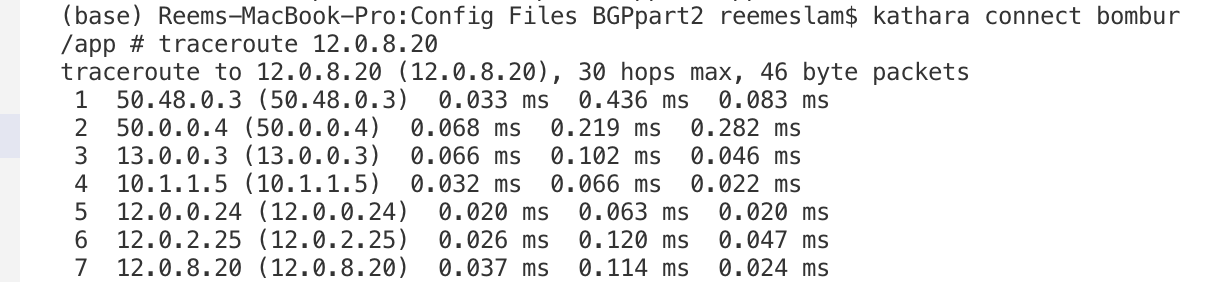
\includegraphics[width=0.73\textwidth]{Images/traceR2BomToBalin.png}
  \caption{Traceroute from bombur to balin}
  \label{fig:2.21}
\end{figure}


\section{Start a Wireshark capture on the involved CD I or W and remember if rip1 or rip4 are traversed.}
In this section we are supposed to capture traffic on collision domain I or W.
\\ There is a problem in capturing by wireshark in macbook from Kathara lab so I tried to use tcpdump but unfortunately the image doesnot recognise tcpdump.
hence we could not attach the required screenshot in this section.

\section{Checking TTL change}
\subsection{Contentiously ping balin from bombur }
\begin{figure}[H]
\centering
  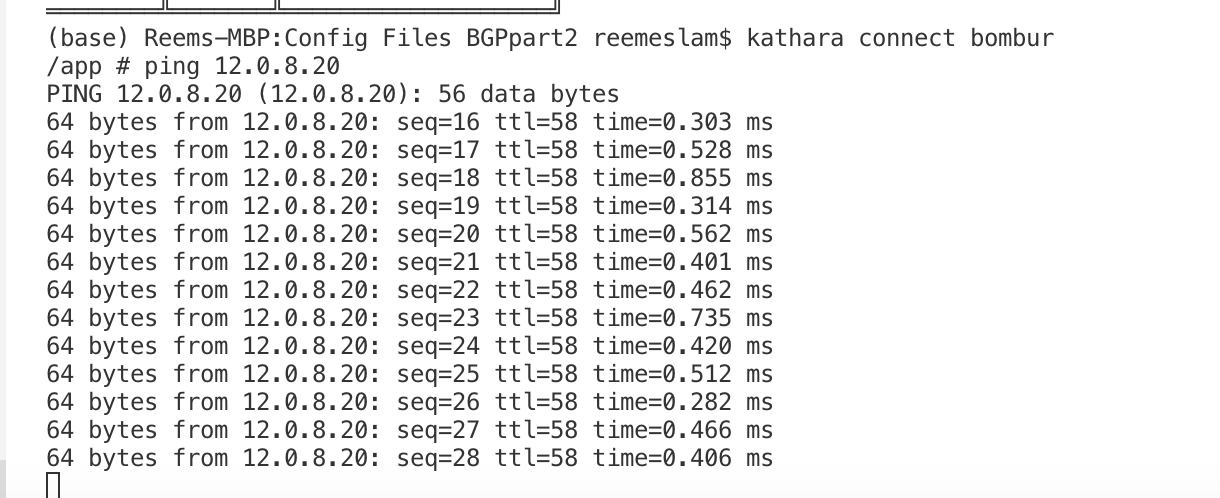
\includegraphics[width=0.73\textwidth]{Images/pingFromBomTobal.png}
  \caption{Contenious ping from Bombur to Bali}
  \label{fig:2.22}
\end{figure}
\subsection{Open Vtysh terminal in Rip4 and shutdown neighbor core3 }
\begin{figure}[H]
\centering
  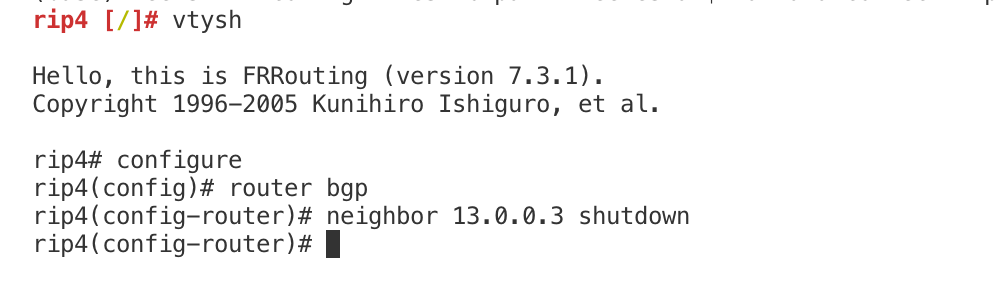
\includegraphics[width=0.73\textwidth]{Images/rip4ShutDownCore3.png}
  \caption{Shutdown core3 as neighbor from rip4 BGP}
  \label{fig:2.23}
\end{figure}
\subsection{Checking TTL change}
Ttl did not change and ping have stopped which should not be the case but I do not know why it stopped
\begin{figure}[H]
\centering
  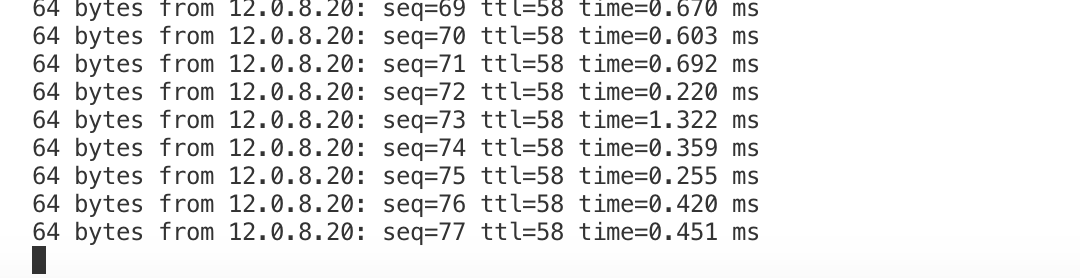
\includegraphics[width=0.73\textwidth]{Images/wrongATT.png}
  \caption{Pinging have stopped instead of Ttl change !}
  \label{fig:2.24}
\end{figure}
\subsection{Enable core3 again as neighbor in rip4}
\begin{figure}[H]
\centering
  
\includegraphics[width=0.73\textwidth]{Images/enableCor3Again.png}
  \caption{Enable core3 as neighbor in rip4}
  \label{fig:2.24}
\end{figure}
There is a problem in capturing by wireshark in macbook from Kathara lab so I tried to use tcpdump but unfortunately the image doesnot recognise tcpdump.
hence we could not attach the required screenshot for wireshark in this section.

